\documentclass[../main.tex]
		
\begin{document}
\section{Predicate logic and Quantifiers}
	\begin{description}
		\item[Task:] Understand enough predicate logic to make sense of quantified statements.
		\item In predicate logic, propositions depend on variable x, y, z, so their truth value may change depending on which values these variables assume: $P(x), Q(x, y), R(x, y, z)$
	\end{description}
	Jargon: domain of discourse(domain)
	
	\subsection{Introduce quantifiers}
	\subsubsection{$\exists$ existential quantifier}
	\begin{description}
		\item[Syntax:] $\exists xP(x)$
		\item[Definition:] $\exists xP(x)$ is true if $P(x)$ is true or some value of $x$; it is false otherwise.
	\end{description}
	
	\subsubsection{$\forall$ universal quantifier}
	\begin{description}
		\item[Syntax:] $\forall xP(x)$
		\item[Definition:] $\forall xP(x)$ is true if $P(x)$ is true for all allowable values of $x$. It is false otherwise.
	\end{description}
	
	\subsubsection{$\exists!$ for one and only one: Uniqueness Quantifier}
	\begin{description}
		\item[Syntax:] $\exists! xP(x) or \exists_{1}$
		\item[Definition:] $\exists! xP(x)$ is true if $P(x)$ is true for exactly one value of $x$ and false for all often values of $x$; otherwise, $\exists! xP(x)$ is false.
	\end{description}
	
	\subsubsection{Alternation of Quantifiers: Nested Quantifiers}
	\begin{tabular}{lr}
		$\forall x\exists y\forall z$ & $P(x, y, z)$ \\
	\end{tabular}
	~\\
	\textbf{NB:} The order \underline{cannot} be exchanged as it might modify the truth values of the statement (think of examples with two quantifiers).
	\begin{description}
		\item[Example:]domain: real numbers, P(x,y):= x + y = y + x\newline$\forall x \forall yP(x,y) \equiv \forall y \forall xP(x,y) $ 
	\end{description}
	
	\subsubsection{Negation of Quantifiers}
	\begin{tabular}{rcl}
		$\lnot(\exists xP(x))$ & $\leftrightarrow$ & $\forall x\lnot P(x)$ \\
		$\lnot(\forall xP(x))$ & $\leftrightarrow$ & $\exists x\lnot P(x)$ \\
	\end{tabular}
	\subsubsection{Precedence of Quantifiers}
	The quantifiers $\forall$ and $\exists$ have higher precedence than all logical operators from propositional calculus.
	$\forall xP(x) \vee Q(x) \equiv (\forall xP(x))\vee Q(x)\\$
	When the domain of a quantifier if finite, quantified statements can be expressed using propositional logic.

	\subsubsection{Order of Quantifiers}
	\begin{description}
		\item[$\forall \forall$:] The order of nested universal quantifiers in a statement without other quantifiers can be changed without changing the meaning of the quantified statement.
		\newline Like x,y real numbers, P(x,y):= x + y = y + x, s.t. $\forall x \forall yP(x,y) \equiv \forall y \forall xP(x,y)$
		\item[$\forall \exists$/$\exists \forall$:]  Like x,y real numbers, Q(x,y):= x + y = 0\\$~~\forall x \exists yQ(x,y):$ y can depend on x; $\exists y \forall x:$ y is a constant independent of x. It's like the order {$\forall,\exists,...$}from the smallest scope to the largest scope.
	\end{description}

	\subsubsection{Null Quantifiers}
	$(\forall xP(x)) \vee A \equiv\forall x(P(x)\vee A)~~~~(\exists xP(x)) \vee A \equiv\exists x(P(x)\vee A)$\newline
	$(\forall xP(x)) \wedge A \equiv\forall x(P(x)\wedge A)~~~~(\exists xP(x)) \wedge A \equiv\exists x(P(x)\wedge A)$\newline
	$(\forall xP(x)) \wedge A \rightarrow\forall x(P(x)\wedge A)~~~(\exists xP(x)) \wedge A \rightarrow\exists x(P(x)\wedge A)$
	
	
	\subsection{Binding variables}
	\begin{description}
		\item[bound:] A quantifier is used on a variable x, which we say x is $\textbf{bound}$
		\item[free:] No quantifier or set bounds a variable, which we say x is $\textbf{free}$
		\item[scope:] The part of a logical expression a quantifier is applied, which we say the part is the $\textbf{scope}$ of the quantifier
		\item[Binding variables:] the same letter is often used of represent variables bound by different quantifiers with scopes that do $\textbf{not overlap}$.\\Substitution: $\exists(P(x)\wedge Q(x))\vee \forall yR(y) ~\stackrel{y\rightarrow x}{\longrightarrow}~ \exists(P(x)\wedge Q(x))\vee \forall xR(x)$ 
	\end{description}
	\subsection{Logical Equavalences Involving Quantifiers}
	\begin{description}
		\item[Distributive Law:] $\newline$ $\forall x(P(x)\wedge Q(x))\equiv \forall xP(x) \wedge \forall xQ(x)$ \newline$\exists x(P(x)\vee Q(x))\equiv\exists xP(x) \vee\exists xQ(x)$
	\end{description}

	\subsection{Rules of Inference}
	\begin{description}
		\item[argument: ]a sequence of statements that end with a conclusion
		\item[valid: ]  the conclusion must follow from true  \textbf{premises} or a tautology
		\item[fallacy: ] leads to invalid argument, some forms of incorrect resoning 
	\end{description}
	\begin{figure}[!htbp]
		\centering
		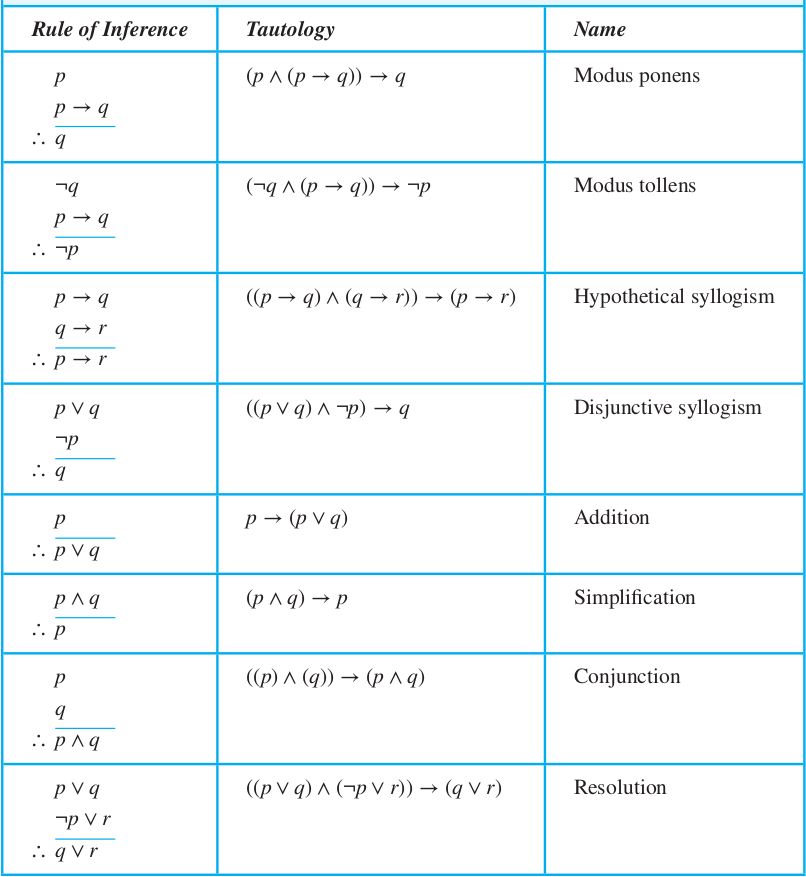
\includegraphics[scale=0.25]{../Figure/pic4.png}
		\caption{Rule of Inference}
	\end{figure}
	\begin{description}
		\item[Constructive dilemma: ] $(A\Rightarrow B), (C\Rightarrow D), (A\vee C) \Leftrightarrow (B\vee D)$
		\item[Clauses: ] To construct proofs in propositional logic using resolution as the only rule of 
		inference, the hypotheses and conclusion must be expressed as \textbf{clauses}, 
		where a clause is a disjuction of variables or negations of these variables.
		\item[Example of Resolution: ]Premises$(p\wedge q)\vee r$, $r\rightarrow s$, conclusion $p\vee s$
	\end{description}

	\subsubsection{Rules of Inference for \textcolor{orange}{Quantified Statements}}
	\begin{description}
		\item[(UI)Universal instantiation: ] "All women are wise" that "Lisa is wise", where Lisa is a member of the domain of all women.
		\item[(UG)Universal generalization: ] The premise $c$ must arbitrarily picked without additional assumptions.
		\item[(EI)Existential instantiation: ] We have no knowledge of what $c$ is, only that is exists. Because it exists, we may give it a name ($c$) and continue the argument.
		\item[(EG)Existential generalization: ] We know one element $c$ in the domain for which p($c$) is true, then we know that $\exists xP(x)$ is true.
	\end{description}
	\begin{figure}[!htbp]
		\centering
		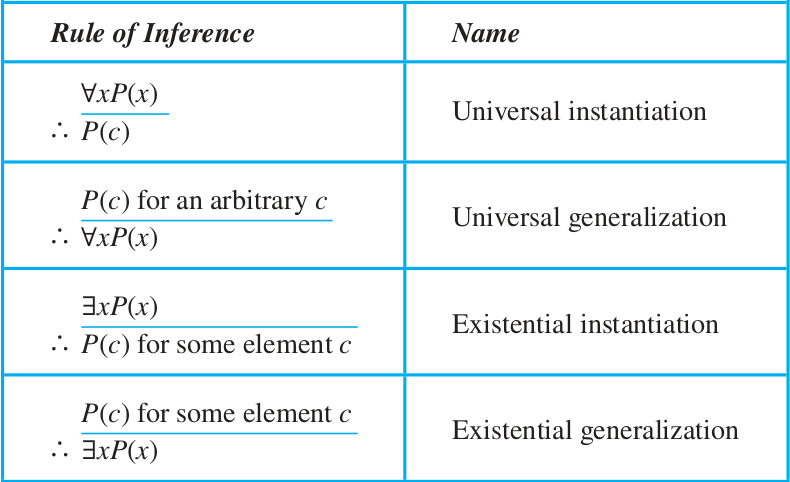
\includegraphics[scale=0.25]{../Figure/pic5.png}
		\caption{Rule of Inference for Quantified Statements}
	\end{figure}
	

\end{document}